\section{Introduction}\label{sec:intro}

\fablenote{Venue mechanics: this source is in ACL ARR format. AAAI requires the \texttt{aaai} style files (two-column, 7 pages + references for the main track), AAAI-style anonymization, and a reproducibility checklist. Convert the template before any submission; the Limitations section is optional at AAAI and can be folded into the conclusion or kept as a subsection to save space.}

% -----------------------------------------------------------------------
% REWRITTEN INTRODUCTION — NLP-first framing for EMNLP
% -----------------------------------------------------------------------

Consider two questions posed about the same image: \emph{``Is there a car in the photo?''} and \emph{``What does the license plate say?''}
The first can be answered from a heavily compressed thumbnail; the second requires reading fine-grained text at full resolution.
This distinction---\emph{what visual fidelity a question demands}---is not random: questions containing words like \emph{how many}, \emph{what color}, \emph{read the text}, or \emph{which airline} signal subtasks (counting, color discrimination, OCR, logo recognition) that require high-resolution evidence, while questions containing \emph{is there}, \emph{does the image show}, or \emph{what type} are typically resolvable from low-fidelity representations.
We show that this linguistic predictability is strong enough to drive a principled pre-retrieval fidelity selection system, enabling significant cost reductions with a controllable accuracy--cost trade-off.
\fablenote{Two issues. (1) ``without sacrificing answer quality'' contradicts your own results (average 10-point gap on general VQA); a reviewer who reads Table~1 after this sentence will distrust the rest of the paper. Say ``with a controllable accuracy--cost trade-off'' instead. (2) For AAAI, add one sentence here casting the problem in decision-theoretic terms: this is sequential information acquisition under cost, an instance of value-of-information reasoning (Howard 1966) --- AAAI reviewers reward papers that name their problem class precisely.}

Despite this predictability, most VLMs retrieve images at a fixed resolution regardless of the query~\cite{alayrac2022flamingo, li2023blip2, liu2024visual, bai2023qwen}.
Model routing methods~\cite{chen2023frugalgpt, ding2024hybrid, wang2024routellm} reduce inference cost but make their decision \emph{after} context is retrieved, assuming all fidelities are freely accessible.
In practice, images are stored across heterogeneous tiers at different retrieval costs~\cite{lonn2019smartphonepictureorganizationhierarchical, aws_s3_storage_classes}; retrieval cost is incurred \emph{before} any model runs, so post-hoc routing cannot avoid it.
Concurrent resolution-selection work~\cite{kimhi2025cares} still requires running a compact VLM on the image; \textsc{VOILA} routes from question text \emph{before any image is accessed}.


\begin{figure}[tb]
    \centering
    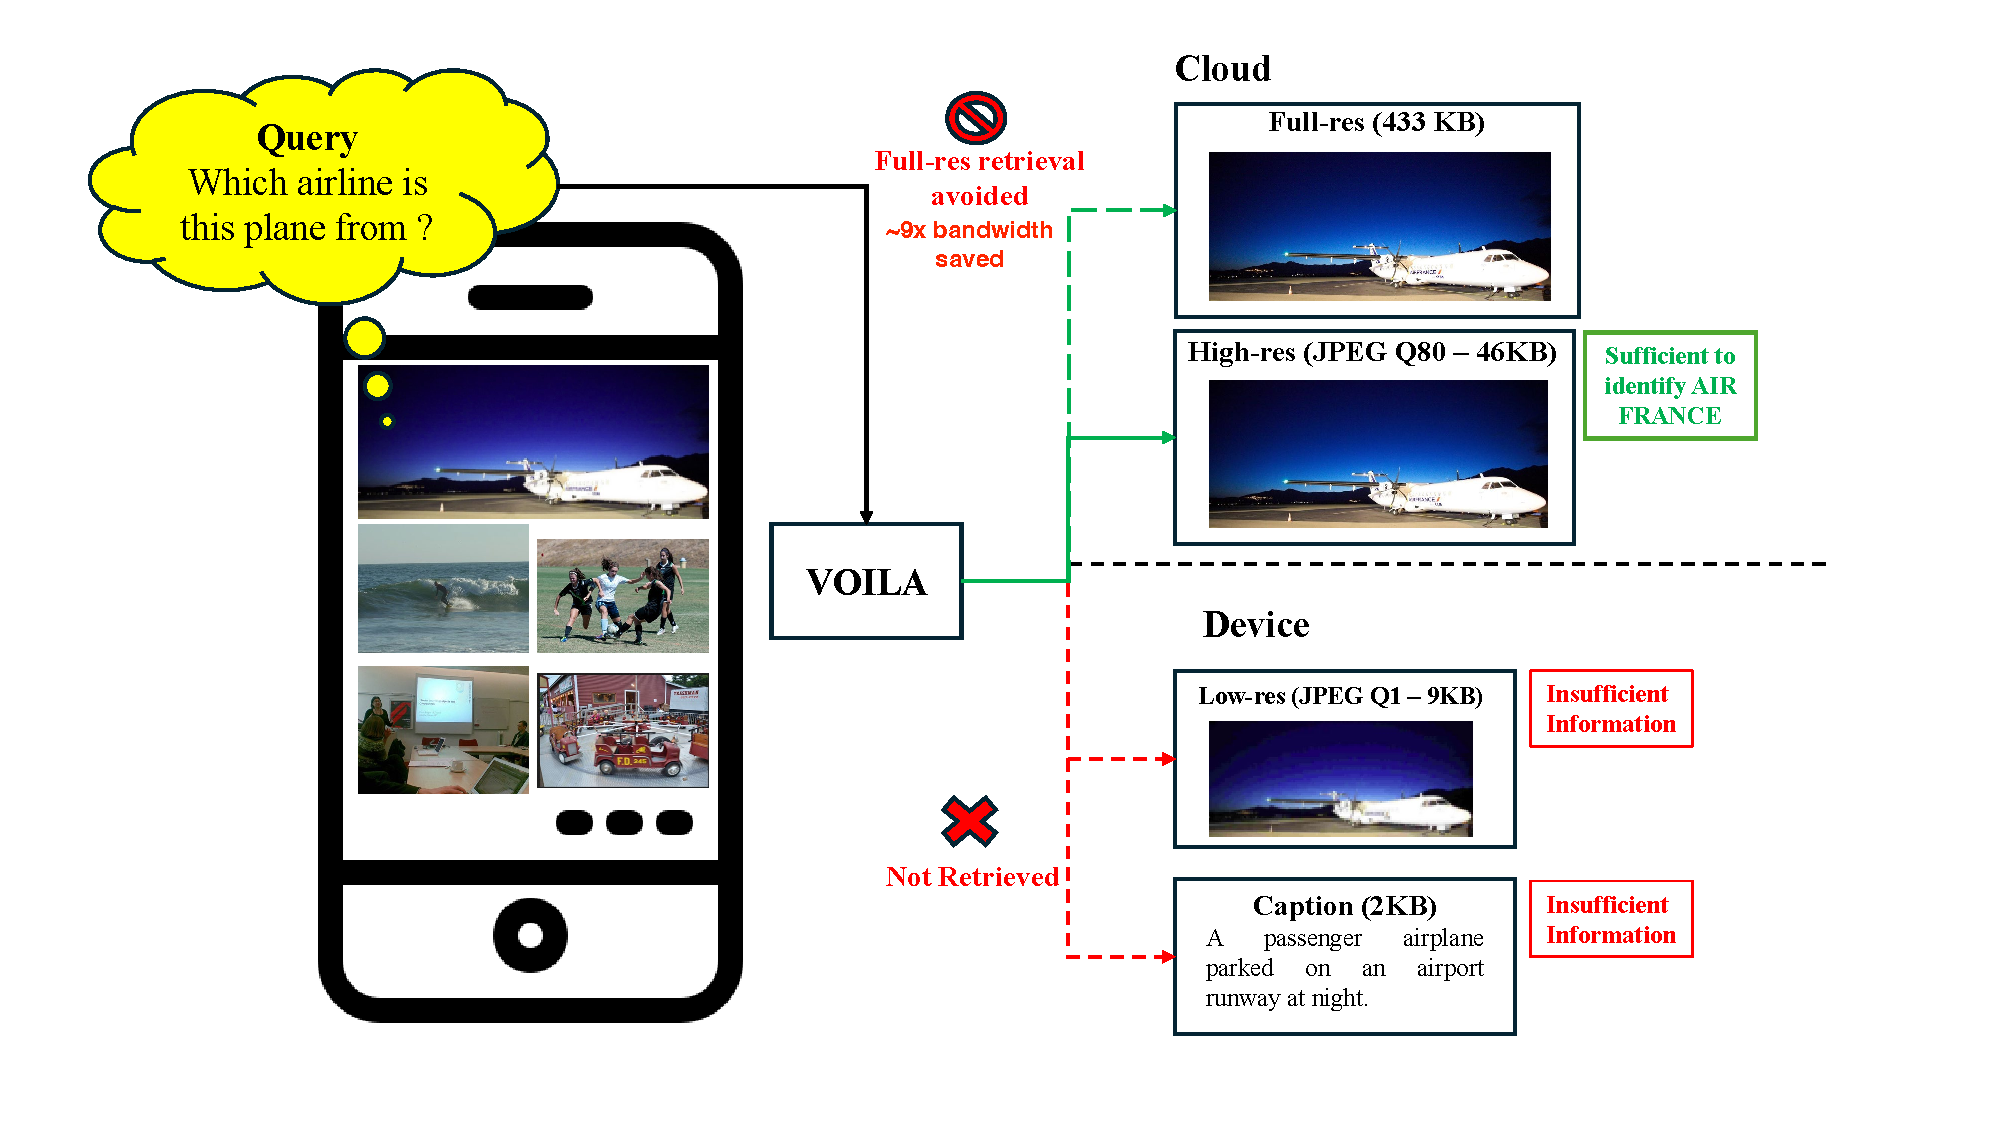
\includegraphics[width=0.9\linewidth]{figures/voila_overview.pdf}
    \caption{VOILA predicts the minimum visual fidelity required to answer a query \emph{before} any image is retrieved. For ``Which airline is this plane from?''---an OCR-dependent question---VOILA selects a mid-fidelity JPEG (46 KB) that preserves the airline logo, avoiding full-resolution retrieval (433 KB) and achieving a 9$\times$ bandwidth reduction.}
    \label{fig:obs1}
\end{figure}

\begin{figure*}[h]
    \centering
    \subfloat[Each curve traces accuracy vs.\ fidelity for one question type; stars mark the first fidelity achieving 95\% of full-resolution accuracy. Counting and OCR tasks require full resolution; yes/no and color saturate at JPEG Q10 (cost 53.2).\label{fig:obs1_dist}]{%
        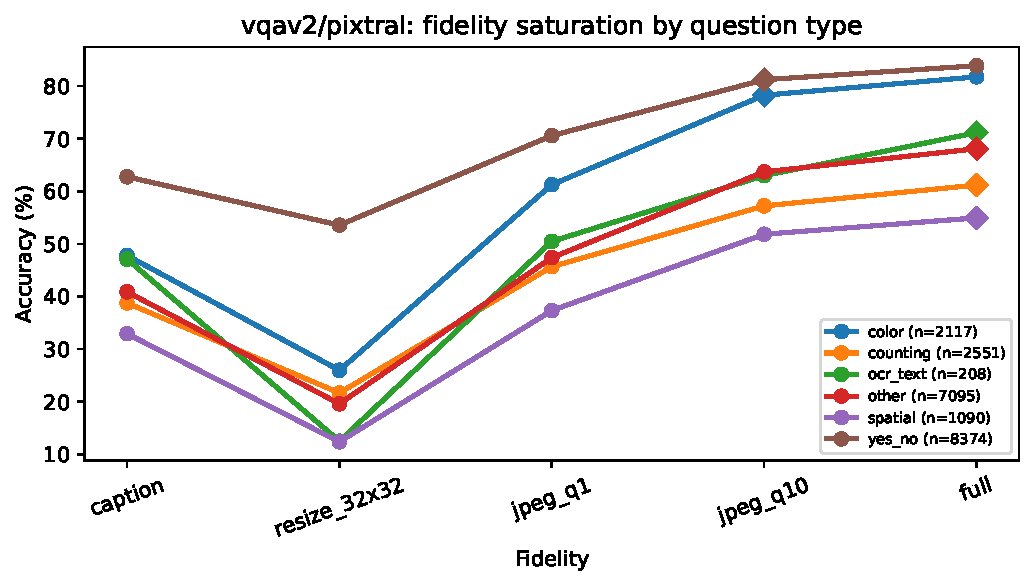
\includegraphics[width=0.32\linewidth]{plots/fidelity_saturation_vqav2_pixtral.pdf}
    }
    \hfill
    \subfloat[VLM output log-probabilities are unreliable indicators of context sufficiency: incorrect low-fidelity answers receive confidence scores comparable to correct ones.\label{fig:obs2_confidence}]{%
        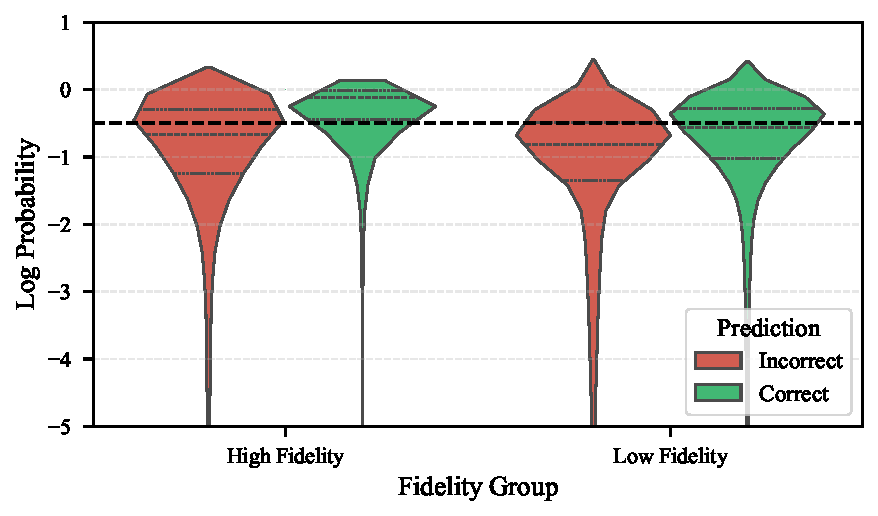
\includegraphics[width=0.32\linewidth]{plots/logprob_collapsed_fidelity_comparison.pdf}
    }
    \hfill
    \subfloat[Model scaling does not compensate for insufficient fidelity: accuracy saturates or degrades at low fidelity regardless of model size.\label{fig:model_scaling_fidelity}]{%
        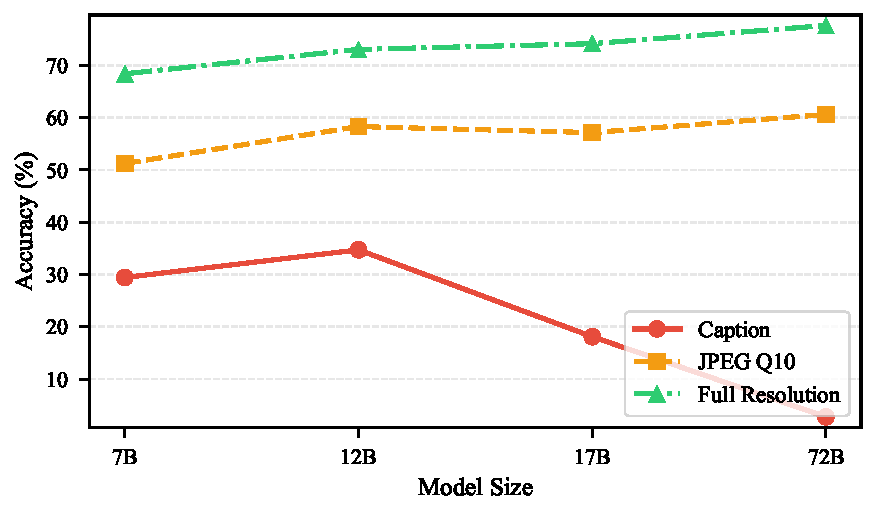
\includegraphics[width=0.32\linewidth]{plots/model_scaling_fidelity_accuracy.pdf}
    }
    \caption{Three empirical observations on VQA-v2 with Pixtral-12B that motivate VOILA's design: (a) question type reliably predicts fidelity requirements; (b) post-hoc confidence signals are unreliable for escalation decisions; (c) model scaling cannot substitute for adequate visual information.}\label{fig:observations_combined}
\end{figure*}

We formalize this as \emph{pre-retrieval fidelity selection} and introduce \textbf{VOILA} (\underline{V}alue-\underline{O}f-\underline{I}nformation guided \underline{L}atency-\underline{A}ware fidelity selection): a gradient-boosted classifier over question features estimates per-fidelity correctness probabilities, isotonic calibration converts raw scores into reliable probabilities, and a greedy value-of-information rule selects the minimum-cost sufficient fidelity---all before any retrieval cost is incurred, with regret bounded by calibration error (Appendix~\ref{sec:theory}).

This paper makes the following contributions:

\begin{itemize}[nosep]
    \item \textbf{Problem formulation:} Pre-retrieval fidelity selection for multimodal RAG---distinct from post-retrieval cascades and from concurrent methods that still require image access---with a near-Bayes-optimal greedy policy under calibrated estimation (\S\ref{sec:method}, Appendix~\ref{sec:theory}).

    \item \textbf{Empirical finding:} Question linguistic structure (\emph{how many}, \emph{what color} vs.\ \emph{is there}, \emph{does it show}) is a strong, sufficient signal for fidelity routing without image access (\S\ref{sec:background}).
    \fablenote{``sufficient'' overclaims: your own error analysis shows 23--25\% under-escalation where linguistic structure does NOT determine the right fidelity. Write ``strong and practically useful'' and explicitly acknowledge the residual visual-context dependence --- pre-empting the obvious counterexample (``How many people?'' over a crowd vs.\ two people) makes the claim more credible, not less.}

    \item \textbf{VOILA framework:} A model-agnostic GBR\,+\,isotonic-calibration system running in 0.45\,ms per query on CPU, with no VLM involvement at decision time (\S\ref{sec:method}).

    \item \textbf{Evaluation} across six VLMs (7B--235B) and five datasets: 50--65\% cost reduction, matching or exceeding full-resolution on OCR-heavy and specialized benchmarks, within 10 accuracy points (average) on general VQA.
\end{itemize}

\fablenote{Contribution list polish for AAAI: (1) the theory (near-Bayes-optimality, regret bounded by calibration error) is currently buried inside the problem-formulation bullet --- AAAI values theory; promote it to its own contribution bullet and state the regret bound informally in one line. (2) The intro never states the headline \emph{against baselines}, only against full-resolution; add ``outperforms log-prob cascades and an LLM router on the accuracy--cost Pareto frontier'' so the contribution is positioned against prior methods, not just a fixed policy. (3) The VOILA acronym is expanded here as ``Latency-Aware'' but the title says ``Fidelity Selection''; make the expansion consistent.}

% -----------------------------------------------------------------------
% OLD INTRODUCTION TEXT (kept for reference)
% -----------------------------------------------------------------------
\begin{comment}
Modern multimodal vision-language systems achieve remarkable accuracy on visual reasoning tasks by scaling models and training data~\cite{alayrac2022flamingo, li2023blip2, liu2024visual}, incurring substantially higher storage, bandwidth, and computational overheads. Recent work has addressed this by focusing on \emph{model selection} and \emph{adaptive routing} -- dynamically choosing between lightweight and heavyweight models based on query characteristics~\cite{chen2023frugalgpt, ding2024hybrid, wang2024routellm}. While reducing \emph{inference costs}, these approaches implicitly assume that input context is fixed and freely available.

In practice, this assumption rarely holds. Multimodal inputs often reside across heterogeneous storage tiers with varying retrieval latencies and costs. Mobile services like Google Photos and iCloud Photos store images at multiple resolutions: on-device caches contain compressed thumbnails and captions, while full-resolution originals reside in cloud storage~\cite{lonn2019smartphonepictureorganizationhierarchical, toderici2016variablerateimagecompression}. Similarly, enterprise systems use hot storage (e.g., AWS S3 Standard) for frequently accessed data and cold storage (e.g., AWS Glacier) for archival content, with retrieval latencies measured in minutes to hours~\cite{aws_s3_storage_classes}. Critically, these retrieval costs are incurred \emph{before} any model processes the input, making post-hoc model routing insufficient for end-to-end efficiency.

We argue that \textbf{context selection at the pre-retrieval stage is a distinct and fundamental learning problem}, orthogonal to model routing. Before asking \emph{which model should answer this query?}, we ask: \emph{Which representation of the available context should be retrieved at all}? Figure~\ref{fig:obs1} shows that for ``Which airline is this plane from?'', a VLM cannot answer from a caption (2 KB) but identifies ``Air France'' from a compressed JPEG (46 KB), avoiding full-resolution retrieval (433 KB)—a 9$\times$ reduction. \textbf{Different queries need different fidelities}, predictable before retrieval.
\end{comment}
